\documentclass{standalone}

\usepackage{tikz}

\usetikzlibrary{calc}
\usetikzlibrary{positioning}
\usetikzlibrary{decorations}
\usetikzlibrary{decorations.markings}
\usetikzlibrary{decorations.text}

\begin{document}
  %noformat{
  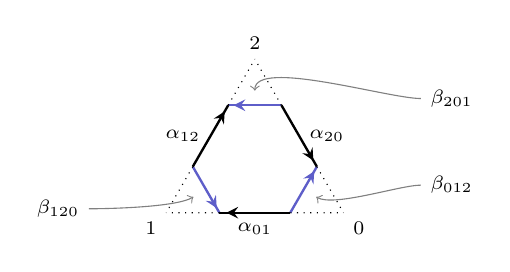
\begin{tikzpicture}
    \tikzstyle{r} = [color=red!70!darkgray!70]
    \tikzstyle{b} = [color=blue!60!darkgray!70]
    \tikzstyle{e} = [postaction=decorate, decoration={markings, mark=at position 0.9 with {\arrow{stealth}}}, line width=0.3mm]

    \tikzset{font=\scriptsize}

    \coordinate[label=330:{$0$}] (v0) at (330:1.3);
    \coordinate[label=210:{$1$}] (v1) at (210:1.3);
    \coordinate[label= 90:{$2$}] (v2) at ( 90:1.3);

    \coordinate (v01) at ($ (v0)!0.3!(v1)  $);
    \coordinate (v02) at ($ (v0)!0.3!(v2)  $);

    \coordinate (v10) at ($ (v1)!0.3!(v0)  $);
    \coordinate (v12) at ($ (v1)!0.3!(v2)  $);

    \coordinate (v20) at ($ (v2)!0.3!(v0)  $);
    \coordinate (v21) at ($ (v2)!0.3!(v1)  $);

    \draw[e, b] (v01) to (v02);
    \draw[e, b] (v12) to (v10);
    \draw[e, b] (v20) to (v21);

    \draw[e] (v01) to node[pos=0.5, below] (a01) {$\alpha_{01}$} (v10);
    \draw[e] (v20) to node[pos=0.5, right] (a20) {$\alpha_{20}$} (v02);
    \draw[e] (v12) to node[pos=0.5, left ] (a12) {$\alpha_{12}$} (v21);

    \draw[dotted] (v01) to (v0);
    \draw[dotted] (v02) to (v0);

    \draw[dotted] (v10) to (v1);
    \draw[dotted] (v12) to (v1);

    \draw[dotted] (v20) to (v2);
    \draw[dotted] (v21) to (v2);

    \node (b012) at ($ (  0:2.5) + (270:0.3) $) {$\beta_{012}$};
    \node (b120) at ($ (180:2.5) + (270:0.6) $) {$\beta_{120}$};
    \node (b201) at ($ (  0:2.5) + ( 90:0.8) $) {$\beta_{201}$};
    \draw[->, looseness=0.5, gray] (b012) to[out=180, in=330] (330:0.9);
    \draw[->, looseness=0.5, gray] (b201) to[out=180, in= 90] ( 90:0.9);
    \draw[->, looseness=0.5, gray] (b120) to[out=  0, in=210] (210:0.9);
  \end{tikzpicture}
  %}noformat
\end{document}
